%!TEX TS-program = xelatex 
%!TEX encoding = UTF-8 Unicode

\documentclass[ignorenonframetext, t]{beamer}
%\documentclass[a4paper]{article}
%\usepackage{beamerarticle}
\usepackage{thucourse}
\includeonlyframes{current}

\title{光阴极物理}
\subtitle{高亮度电子束物理及应用}
\author{唐传祥}
\institute{清华大学工程物理系}
\date{2016--2017 秋季学期}

\begin{document}

\begin{frame}
  \titlepage
\end{frame}

\begin{frame}
  \frametitle{目录}
  \begin{multicols}{2}
  \tableofcontents
	\end{multicols}
\end{frame}

\section{光电效应}

\subsection{光电效应基础知识}

\begin{frame}
  \frametitle{光电效应的基本概念}
  \begin{concept}
  	\alert{光电效应}是指光束照射在金属表面会使其发射电子的物理现象,发射出的电子被称为\alert{光电子}。
	\end{concept}
%	\begin{center}
%		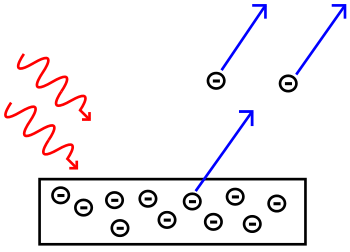
\includegraphics[width=0.3\linewidth]{photoelectric}
%	\end{center}
  \begin{itemize}
	  \item 对于特定金属而言,入射光频率必须大于某特定值才能产生光电效应,光电效应的发生与否与入射光强度没有关系
	  \item 光电效应是一种量子效应,无法用 Maxwell 体系的经典电磁理论解释,必须借助\alert{光量子}的概念才能解释
	  \item 光电效应可用下面著名的公式描述:
	  \begin{formula}{光电效应光电子最大能量}
	  \[
	  E = h\nu-\phi
	  \]
	  \scriptsize{其中$E$是出射光电子最大能量,$h\nu$为入射光子能量,$\phi$称为金属的逸出功或功函数(work function)}
	  \end{formula}
  \end{itemize}
\end{frame}

\begin{frame}
  \frametitle{光电效应研究的里程碑}
  \begin{itemize}
	  \item 1887 年 H. Hertz 发现用紫外线照射金属电极会更容易产生电火花,当时被称为赫兹效应,这是实验上首次发现光电效应
	  \item 1899 年 J. Thomson 实验验证了电子的存在
	  \item 1902 年 P. Lenard 实验定性发现出射电子能量与入射光频率正相关,而与入射光强度无关,这与 Maxwell 提出的光的波动理论矛盾
		\item 1905 年 A. Einstein 发文提出光量子概念解释光电效应的实验现象
		\item 1914 年 R. Millikan 实验验证了 Einstein 的光电效应公式
  \end{itemize}
\end{frame}

\subsection{单光子/多光子光电效应}

\begin{frame}
	\frametitle{单光子光电效应}
	\begin{concept}
  	\alert{单光子光电效应}就是金属内电子吸收单个光子的光电效应。
	\end{concept}
	\only<1>{
	\begin{physics}
		金属内处于费米能级(Fermi Energy)以下的束缚态电子吸收单个光子跃迁到高能态,进而成为自由电子向四周运动;经过若干次散射(能量损失)后部分高能态电子会到达金属表面,其中又有部分电子具有足够能量,克服金属表面势垒后从金属表面逸出,成为光电子。
	\end{physics}}
	\only<2>{
  \begin{itemize}
	  \item 光电子数目(光电子产额)与入射光强度成正比,因此又被称为线性光电效应,可以定义光阴极的量子效率 QE 如下:
	  \begin{formula}{量子效率定义}
	  \[
	  QE = \frac{N_e}{N_p} = \frac{Q/e}{IS\tau/h\nu} = \frac{Q}{I}\cdot\frac{h\nu}{eS\tau}
	  \]
	  \scriptsize{其中$N_e$为出射光电子数,$N_p$为入射光子数,$Q$是出射束团电荷量,$I$是入射光强度,$h\nu$为入射光子能量,$e$为电子电荷量,$S$为入射光横向面积,$\tau$为入射光脉宽}
	  \end{formula}
	  \item 入射光子能量必须高于金属的逸出功才可以发生单光子光电效应
  \end{itemize}}
\end{frame}

\begin{frame}
	\frametitle{多光子光电效应}
	\begin{concept}
  	\alert{多光子光电效应}就是金属内电子吸收多个光子的光电效应。
	\end{concept}
	\only<1>{
	\begin{physics}
		金属内处于费米能级以下的束缚态电子同步或非同步吸收多个光子跃迁到高能态,进而成为自由电子向四周运动;经过若干次散射(能量损失)后部分高能态电子会到达金属表面,其中又有部分电子具有足够能量,克服金属表面势垒后从金属表面逸出,成为光电子。
	\end{physics}}
	\only<2>{
  \begin{itemize}
	  \item 光电子产额与入射光强度成幂函数关系,因此又被称为高阶光电效应或非线性光电效应;N光子光电效应的光电流密度J与入射光强度I成N次幂关系:
	  \[
	  J \propto I^N
	  \]
	  \item 入射光子能量小于金属逸出功也可能发生多光子光电效应
	  \item 入射光照射金属时会同时发生多个高阶光电效应
	  \item 高阶光电效应的光电子产额随阶数的增大迅速衰减
  \end{itemize}}
\end{frame}

\subsection{零阶光电效应}

\begin{frame}
	\frametitle{热发射}
	\begin{concept}
  	\alert{热发射}即因金属表面电子热运动而产生的电子发射。
	\end{concept}
	\only<1>{
	\begin{physics}
		对于温度高于绝对零度的金属,假定其温度为 $T$($T > 0$),由于金属内部的电子能量服从 Fermi-Dirac 分布($T$ 较小时近似 Maxwell-Boltzmann 分布),其拖尾部分的电子处于较高能态,从而具有足够的能量克服金属表面势垒,逸出金属表面。
	\end{physics}
	\begin{formula}{热发射电流密度}
	\[
	J = AT^2\exp\left(-\frac{\phi}{kT}\right)
	\]
	\scriptsize{其中 $A$ 是Richardson常数,约为 \SI{1202}{\micro A.\milli m^{-2}.K^{-2}};$\phi$ 是金属逸出功,$k$ 是 Boltzmann 常数}
	\end{formula}}
	\only<2>{
  \begin{itemize}
	  \item 热发射是光电发射的特例,电子吸收 0 个光子而逸出金属表面,即 0 阶光电发射,电子逃逸是通过热运动完成的
	  \item 热发射电流只与金属温度$T$有关,与入射光强度大小无关
	  \item 金属温度 $T = 0$ 时,热发射电流 $J = 0$;$T > 0$ 时热发射电流 $J > 0$
	  \item 热发射电流的强度很小,在 $T = \SI{300}{K}$ 时热发射电流在 \SI{1}{\micro A} 量级
  \end{itemize}}
\end{frame}

\begin{frame}
	\frametitle{场致发射}
	\begin{concept}
  	\alert{场致发射}即因金属表面存在很强的引出电场而产生的电子发射。
	\end{concept}
	\only<1>{
	\begin{physics}
		当金属表面存在很强的引出电场(即电场线指向金属表面的电场)时,金属表面势垒会被电场拉低,从而金属表面的电子可以通过\alert{量子隧穿}效应穿越表面势垒,逸出金属表面。
	\end{physics}
	\begin{formula}{场致发射电流密度}
	\[
	J = \frac{A\beta^2 E^2}{\phi}\exp\left(-\frac{B\phi^{3/2}}{\beta E}\right)
	\]
	\scriptsize{其中 $E$ 是电场强度,$\beta$ 为场增强因子,$A, B$ 为与金属表面情况有关的参数,可通过实验拟合得到}
	\end{formula}}
	\only<2>{
  \begin{itemize}
	  \item 场致发射是光电发射的特例,电子吸收 0 个光子而逸出金属表面,即 0 阶光电发射,电子逃逸是通过量子隧穿完成的
	  \item 金属温度 $T = 0$ 时,依然有场致发射电流 $J > 0$
		\item 场致发射电流随引出电场的梯度下降而迅速减小,$E = 0$ 时场致发射电流 $J = 0$
  \end{itemize}}
\end{frame}

\subsection{体光电效应与表面光电效应}

\begin{frame}
	\frametitle{体光电效应}
\end{frame}

\begin{frame}
	\frametitle{表面光电效应}
\end{frame}

\section{光阴极电子发射物理模型}

\subsection{光阴极电子发射模型简述}

\begin{frame}
	\frametitle{模型演化}
\end{frame}

\begin{frame}
	\frametitle{唯象理论与量子理论}
\end{frame}

\subsection{金属中的自由电子}

\begin{frame}
	\frametitle{Drude-Sommerfeld 模型}
	\framesubtitle{模型概述}
	Drude-Sommerfeld 模型是一个用于解释固体宏观性质(导电、传热、比热等)的半经典模型,它结合了经典的 Drude 模型与量子力学中的部分观点(例如作用量量子化),虽然简单却取得了巨大成功。
	\begin{background}
	P. Drude 于 1900 年提出了 Drude 模型,该模型的要点为:
	\begin{itemize}
	\item 固体中的电子可看做经典的带电小球
	\item 固体中的原子核可视为极重的几乎静止的大球
	\item 固体中的电子不停地与原子核发生碰撞
	\end{itemize}
	该模型成功导出了固体中电子的运动方程以及固体中的电流密度与局域电场的线性关系,却很大地高估了固体的比热。其根本原因在于该模型的经典本质。A. Sommerfeld 于 1933 年将部分量子力学的观点应用于 Drude 模型,成功地解释了固体的比热,这就是 Drude-Sommerfeld 模型。
	\end{background}
\end{frame}

\begin{frame}
	\frametitle{Drude-Sommerfeld 模型}
	\framesubtitle{金属中电子的能态密度}
	\only<1>{Drude-Sommerfeld 模型中,固体中电子形态为自由电子费米气体(也称为简并电子气),自由电子费米气体的一个重要概念就是\alert{能态密度(Energy Density of States,EDOS)}。\\~\\
	金属中的电子的 EDOS 可以推导如下:}
	\only<-2>{\begin{derivation}
	\only<1>{
	固体中电子能量为:
	\[\varepsilon = \dfrac{\hbar^2k^2}{2m}\]
	固体中波的普遍态密度: 
	\[\rho(k) =\left(\frac{V}{2\pi^2}\right)k^2\]}
	\only<2>{
	考虑到单位体积与电子自旋简并数 2,EDOS 可表示为:
	\[g(\varepsilon) =\dfrac{2}{V}\rho(k)\dfrac{dk}{d\varepsilon}\]
	结合前面两式我们有:
	\[g(\varepsilon) = \frac{1}{2\pi^2}\left(\frac{2m}{\hbar^2}\right)^{3/2}\sqrt{\varepsilon}\]}
	\end{derivation}}
	\only<2>{
	于是我们得到:
	\begin{formula}{金属中电子的能态密度}
	\[g(\varepsilon) = \frac{1}{2\pi^2}\left(\frac{2m}{\hbar^2}\right)^{3/2}\sqrt{\varepsilon}\]
	\end{formula}}
	\only<3>{
	下图展示了金属中电子能态密度与能级的开方正比关系:\\~\\
	\begin{center}
	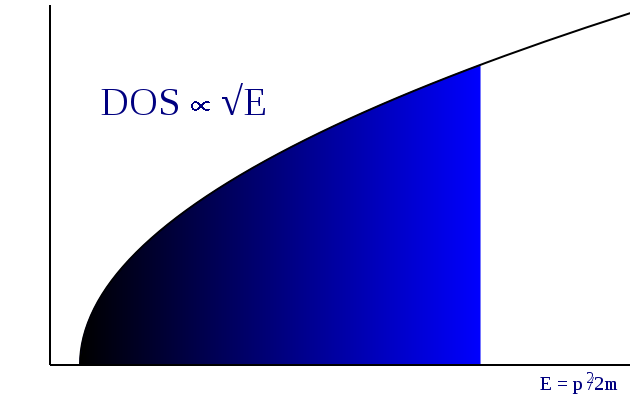
\includegraphics[width=0.5\linewidth]{EDOS}
	\end{center}}
\end{frame}

\begin{frame}
	\frametitle{Drude-Sommerfeld 模型}
	\framesubtitle{金属中电子的速度分布}
	\only<1>{
	量子力学指出,金属中的电子满足 Fermi-Dirac 分布:
	\begin{formula}{Fermi-Dirac 分布}
	\[f(\varepsilon) = \frac{1}{e^{(\varepsilon-\mu)/kT}+1}\]
	\scriptsize{这里 $\varepsilon$ 是能级,$\mu$ 被称为 Fermi 能量,$k$ 是 Boltzmann 常数,$T$ 是金属温度}
	\end{formula}
	Fermi-Dirac 分布描述了金属中的特定能级上的电子占有率。当金属温度 $T\rightarrow \SI{0}{K}$ 时,可以看出对于小于 $\mu$ 的能级电子占有率为 1,大于 $\mu$ 的能级电子占有率为 0。\\~\\
	利用金属中的电子能态密度公式以及 Fermi-Dirac 分布公式,可以得到金属中单位体积电子的速度分布 $n(u, v, w)$。}
	\only<2->{
	\begin{derivation}
	\only<2>{
	金属中单位体积电子的能量分布可写成 $n(\varepsilon)=g(\varepsilon)f(\varepsilon)$,那么有下面等式成立:
	\[\iiint\limits_{\frac{1}{2}m(u^2+v^2+w^2)\in [\varepsilon, \varepsilon+d\varepsilon]}\Zskip\Zskip n(u, v, w)dudvdw = n(\varepsilon)d\varepsilon\]
	假定动量空间均匀分布,那么 $n(u,v,w)=n^{*}\left(\sqrt{u^2+v^2+w^2}\right)$,将 $(u,v,w)$ 变换到球坐标中,积分便可得到:
	\[n(u, v, w) = \dfrac{m^{\frac{3}{2}}}{2\pi\cdot2^{\frac{3}{2}}}\cdot\frac{1}{\sqrt{\varepsilon}}\cdot n(\varepsilon)\]}
	\only<3>{
	代入 $n(\varepsilon)$ 并做变量代换,即得到:
	\[n(u, v, w) = 2\left(\frac{m}{h}\right)^3\frac{dudvdw}{e^{\left[\frac{1}{2}m\left(u^2+v^2+w^2\right)-\mu\right]/kT}+1}\]}
	\end{derivation}}
	\only<3>{
	因此我们得到:
	\begin{formula}{金属中单位体积电子的速度分布}
	\[n(u, v, w) = 2\left(\frac{m}{h}\right)^3\frac{dudvdw}{e^{\left[\frac{1}{2}m\left(u^2+v^2+w^2\right)-\mu\right]/kT}+1}\]
	\end{formula}}
\end{frame}

\subsection{阴极上的空间电荷限}

\begin{frame}[label=current]
	\frametitle{Child-Langmuir 模型}
	\framesubtitle{模型概述}
	Child-Langmuir 模型是研究阴极上\alert{空间电荷限电流(Space-Charge Limited Current, SCLC)}的模型。
	\begin{background}
	C. Child 于 1911 年提出 Child 定律,该定律是说在平行两极板间的电压 $V$ 固定的情况下,其极板间电流密度存在最大值 $J$,并且 $J$ 与 $V$ 成 3/2 次方关系,因此又被称为 3/2 次方定律。1911 年发表的情况针对的是离子流,I. Langmuir 在 1913 年将 Child 的方法应用于电子流,因此该定律又被称为 Child-Langmuir 定律。
	\end{background}
	\begin{physics}
	阴极上空间电荷限的本质是:在两极板间的电流产生的空间电荷场会减小发射极的引出电场,当电流大到一定程度时,发射极表面的总引出电场降到 0,逸出的电子无法获得加速,发射电流无法进一步增加,因此电压固定时发射电流存在饱和值。
	\end{physics}
\end{frame}

\begin{frame}[label=current]
	\frametitle{Child-Langmuir 模型}
	\framesubtitle{稳态情形}
	\only<1>{
	Child-Langmuir 模型的假定如下:
	\begin{itemize}
	\item 不考虑相对论效应
	\item 忽略极板间运动的粒子间的散射
	\item 极板间的粒子是同一的(同质量,同电荷量)
	\item 阴极上的初始发射速度为 0
	\end{itemize}
	那么当两极板间电流处于稳态时,我们可以直接利用 Poisson 方程导出空间电荷限电流公式:}
	\only<-3>{
	\begin{derivation}
	\only<1>{
	我们考虑两极板间电流中的一点,那么有 Poisson 方程成立:
	\[\nabla^2V=-\frac{\rho}{\epsilon_0}\]
	其中 $V$ 为该点电势,$\rho$ 为该点电荷密度。}
	\only<2>{
	由于阴极上($V=0$)粒子的初始动能为 0,根据能量守恒,电势 $V$ 处粒子的能量满足:
	\[\frac{1}{2}mv^2+qV=0\]
	考虑到电荷守恒及稳态条件,有:
	\[\nabla\cdot\vec{J}=-\frac{\partial \rho}{\partial t}= 0\]
	而电流密度$\vec{J}$满足:
	\[\vec{J}=\rho \vec{v}\]}
	\only<3>{
	我们仅考虑一维情形(束流沿 $z$ 轴运动),可知 $J$ 是个常量,联立以上各式可得关于电势 $V$ 的方程:
	\[\frac{d^2V}{dz^2}+AV^{-\frac{1}{2}}=0\]
	其中 $A=-\frac{J}{\varepsilon_0}\sqrt{-m/2q}$。解上面方程并代入边界条件:
	\begin{eqnarray*}
	&&V|_{z=0}=0\\
	&&V|_{z=d}=V_d
	\end{eqnarray*}
	可得电压$V_d$与最大电流密度 $J$ 之间的关系为:
	\[J = \frac{4\varepsilon_0}{9}\sqrt{-2q/m}\cdot \frac{V_d^{\frac{3}{2}}}{d^2}\]}
	\end{derivation}}
	\only<4>{
	对于电子而言,我们就得到阴极上的空间电荷限电流密度为($V_d\rightarrow V$):
	\begin{formula}{阴极的空间电荷限电流密度}
	\[J = \frac{4\varepsilon_0}{9}\sqrt{2e/m}\cdot \frac{V^{\frac{3}{2}}}{d^2}\]
	\end{formula}
	注意上式我们是在平行电极板情形下推导得到的,但是该公式对于圆柱电极板情形也成立,大家可以自己推导一下作为练习。
	\\~\\
	在带有电子枪的电子器件中,人们定义\alert{导流系数$P=I/V^{3/2}$}来衡量电子枪的发射能力,$P$的单位为朴。一般微波器件的电子枪,导流系数在\SIrange[range-phrase = --]{0.1}{1}{\micro P}的范围。导流系数反映了阴极发射电流I与阴阳极间电压V之间的关系,它仅取决于枪的几何尺寸。}
\end{frame}

\begin{frame}[label=current]
	\frametitle{Child-Langmuir 模型}
	\framesubtitle{非稳态情形}
\end{frame}

\subsection{光阴极的热发射电流}

\begin{frame}
	\frametitle{Richardson-Dushman 模型}
\end{frame}

\subsection{光阴极的暗电流}

\begin{frame}
	\frametitle{Fowler–Nordheim 模型}
\end{frame}

\subsection{光阴极的光电流}

\begin{frame}
	\frametitle{Fowler-Dubridge 模型}
	\framesubtitle{单光子光电发射}
\end{frame}

\begin{frame}
	\frametitle{Fowler-Dubridge 模型}
	\framesubtitle{多光子光电发射}
\end{frame}

\subsection{光阴极的量子效率和初始发射度}

\begin{frame}
	\frametitle{Spicer-Dowell 模型}
	\framesubtitle{三步模型}
\end{frame}

\begin{frame}
	\frametitle{Spicer-Dowell 模型}
	\framesubtitle{Schottky 效应和有效逸出功}
\end{frame}

\begin{frame}
	\frametitle{Spicer-Dowell 模型}
	\framesubtitle{光阴极的量子效率}
\end{frame}

\begin{frame}
	\frametitle{Spicer-Dowell 模型}
	\framesubtitle{光阴极的初始发射度}
\end{frame}

\begin{frame}
	\frametitle{Spicer-Dowell 模型}
	\framesubtitle{光阴极的折射定律}
\end{frame}

\subsection{几个量子模型}

\begin{frame}
	\frametitle{Kantorovich-Keldysh 模型}
\end{frame}

\begin{frame}
	\frametitle{Wan 模型}
\end{frame}

\subsection{粗糙表面光阴极上的电子发射}

\begin{frame}
	\frametitle{2D 正弦表面模型}
\end{frame}

\begin{frame}
	\frametitle{\* 3D 任意表面模型}
\end{frame}

\begin{frame}
	\frametitle{\* 纳米精细度模型}
\end{frame}

\section{几种典型的光阴极}

\subsection{传统光阴极}

\begin{frame}
	\frametitle{金属光阴极}
	\framesubtitle{Cu, Mg, Ag}
\end{frame}

\begin{frame}
	\frametitle{半导体光阴极}
	\framesubtitle{PEA 光阴极}
\end{frame}

\begin{frame}
	\frametitle{半导体光阴极}
	\framesubtitle{NEA 光阴极}
\end{frame}

\subsection{几种新型光阴极}

\begin{frame}
	\frametitle{表面等离激元光阴极}
	\framesubtitle{NPC}
\end{frame}

\begin{frame}
	\frametitle{表面等离激元光阴极}
	\framesubtitle{ATR}
\end{frame}

\begin{frame}
	\frametitle{冷阴极}
\end{frame}

\begin{frame}
	\frametitle{复合阴极}
\end{frame}

\end{document}

%\section{Main Part}
%While this text is not shown in the presentation, the section command
%also applies to the presentation.
%We can add a subsection that is only part of the article like this:
%\subsection<article>{Article-Only Section}
%With some more text.
%\begin{frame}
%  This text is part both of the article and of the presentation.
%  \begin{itemize}
%\item This stuff is also shown in both version.
%\item This too.
%  \only<article>{\item This particular item is only part
%      of the article version.}
%  \end{itemize}
%\end{frame}
